\chapter{Software}
\label{chp:S}

%%%%%%%%%%%%%%%%%%%%%%%%%%%%%%%%%%%%%%%%%%%%%%%%%%%%%%%%%%%%%%%%%%%%%%%
\section{Motivation}

Siemens NX 12 is used to create the geometry of the soft elements. NX 12 is very user friendly with simple and easy-to-use interfaces for drawing. NX 12 is capable of exporting geometric files to formats that other FEM software are capable of importing.

MSC.Marc Mentat 2019 is used to model the materials and their behaviour. Marc is capable of advanced non-linear analysis.

Python 3.6 is used to construct a modelling pipeline. Packages are available that allow for the integration of Python, NX 12 and Marc. Many advanced numerical analysis packages are also available for Python.

\section{Approach}

\subsection{Method}

A 5x5 grid of square elements is drawn in NX 12. The geometry is exported to Marc Mentat, where boundary conditions, material properties, and other necessary settings are applied. Boundary conditions are selected as a fixed left and bottom side and a negative pressure ramp exerted on the other surfaces. Figure~\ref{fig:bc} displays the grid and boundary conditions.

\begin{figure}
	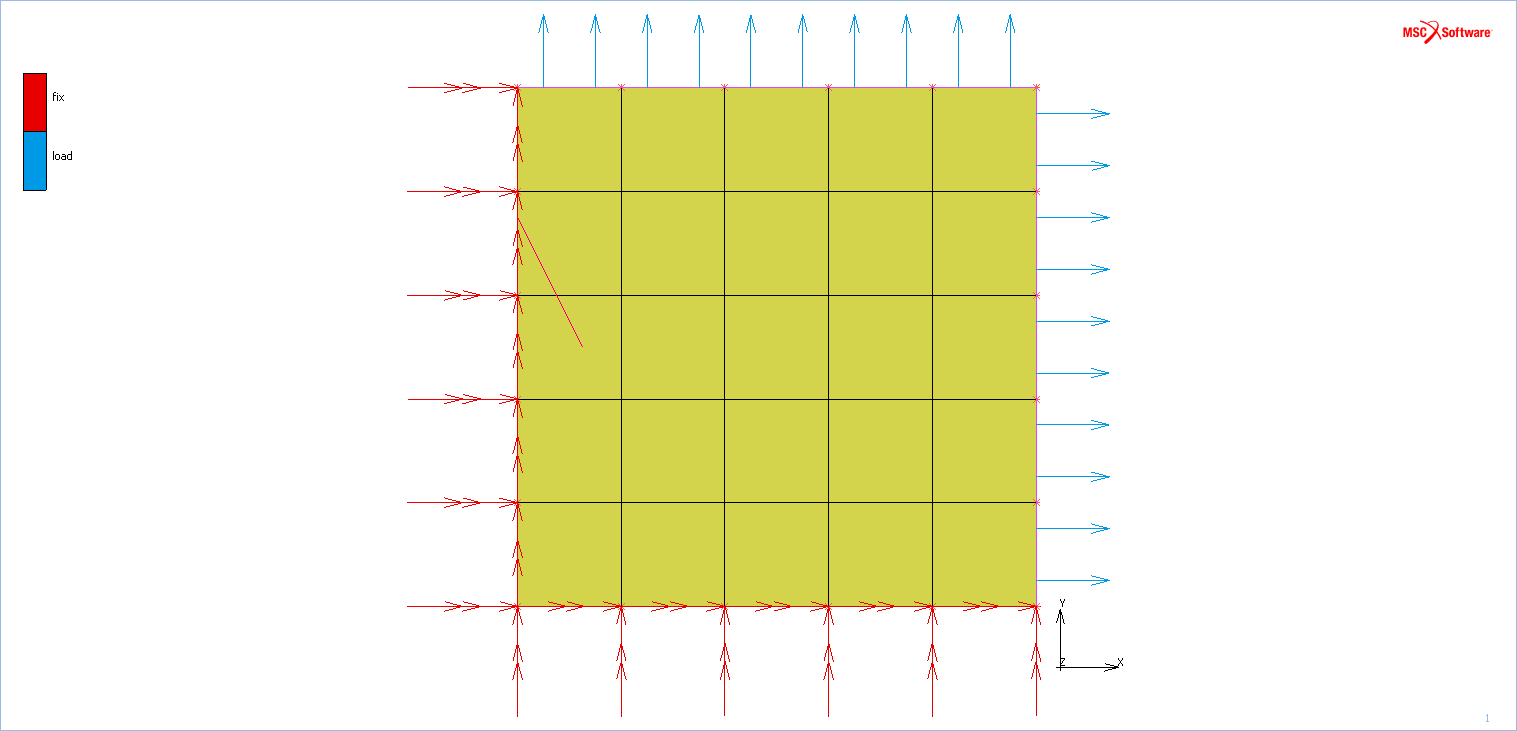
\includegraphics[width=1\textwidth]{baseelement_full_bc.png}
	\caption{Boundary conditions applied to grid of elements}
	\label{fig:bc}
\end{figure}

A random internal element is selected for deletion. The job is run and the results compiled for inspection.

\subsection{Pipeline}

Figure~\ref{fig:fm} displays a flowchart describing the overall pipeline for the creation of the basic soft elements.

\begin{figure}
	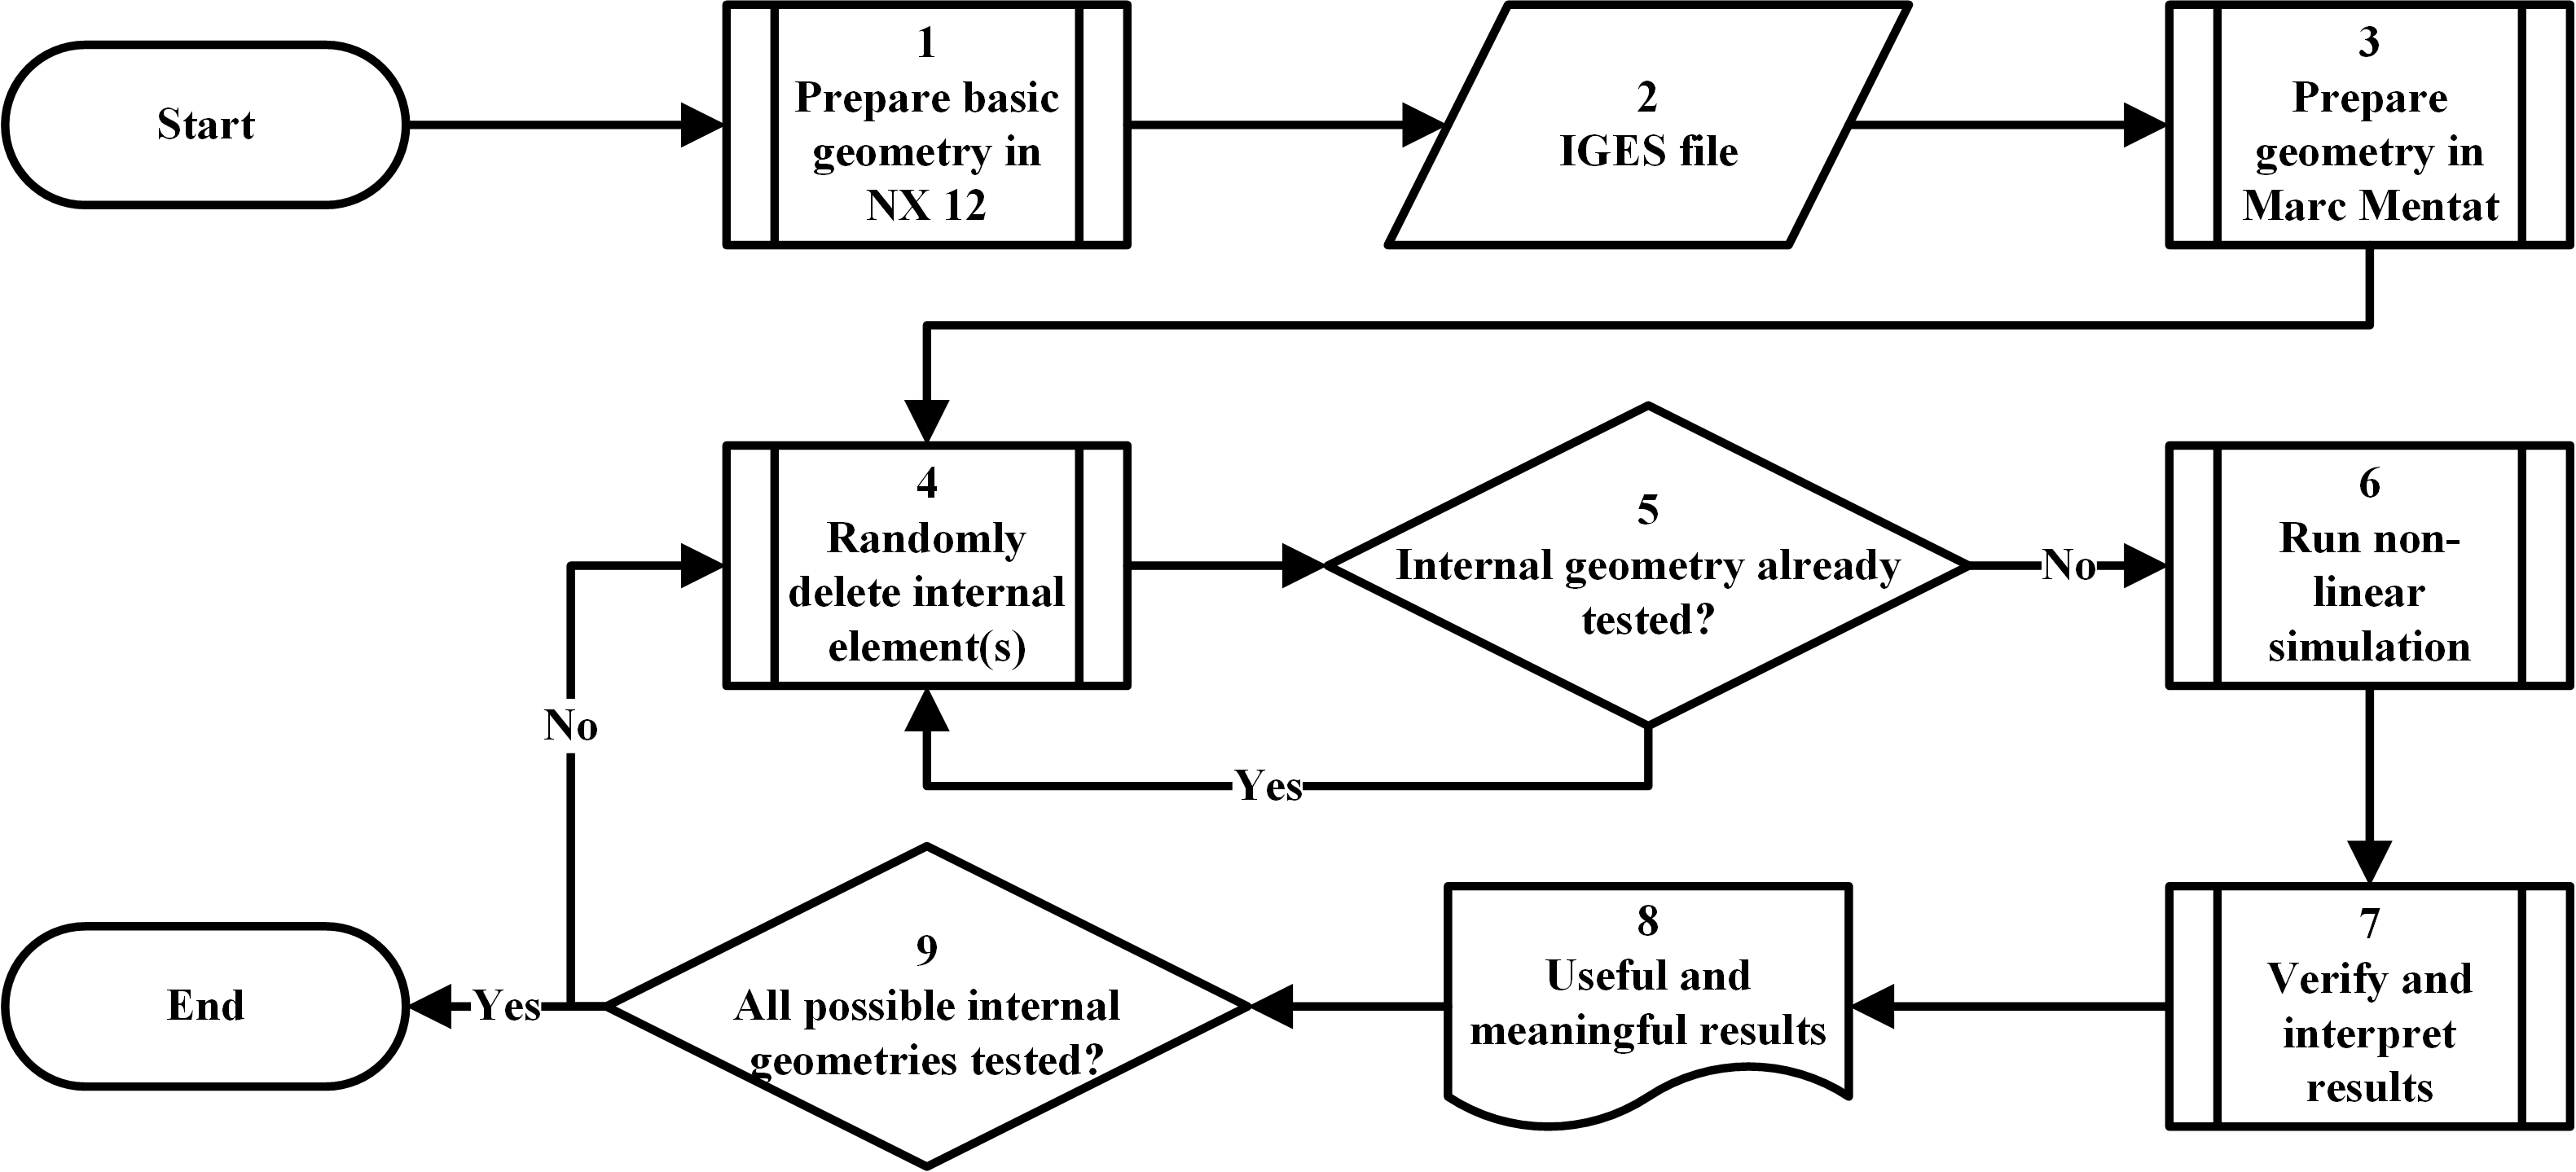
\includegraphics[width=1\textwidth]{Q1_Full.png}
	\caption{Main pipeline flowchart}
	\label{fig:fm}
\end{figure}

Figures~\ref{fig:f1} through~\ref{fig:f7} display the flowcharts elaborating on parts of the pipeline. Tables detailing the exact commands and inputs used in Marc follow the relevant figures.

\begin{figure}
	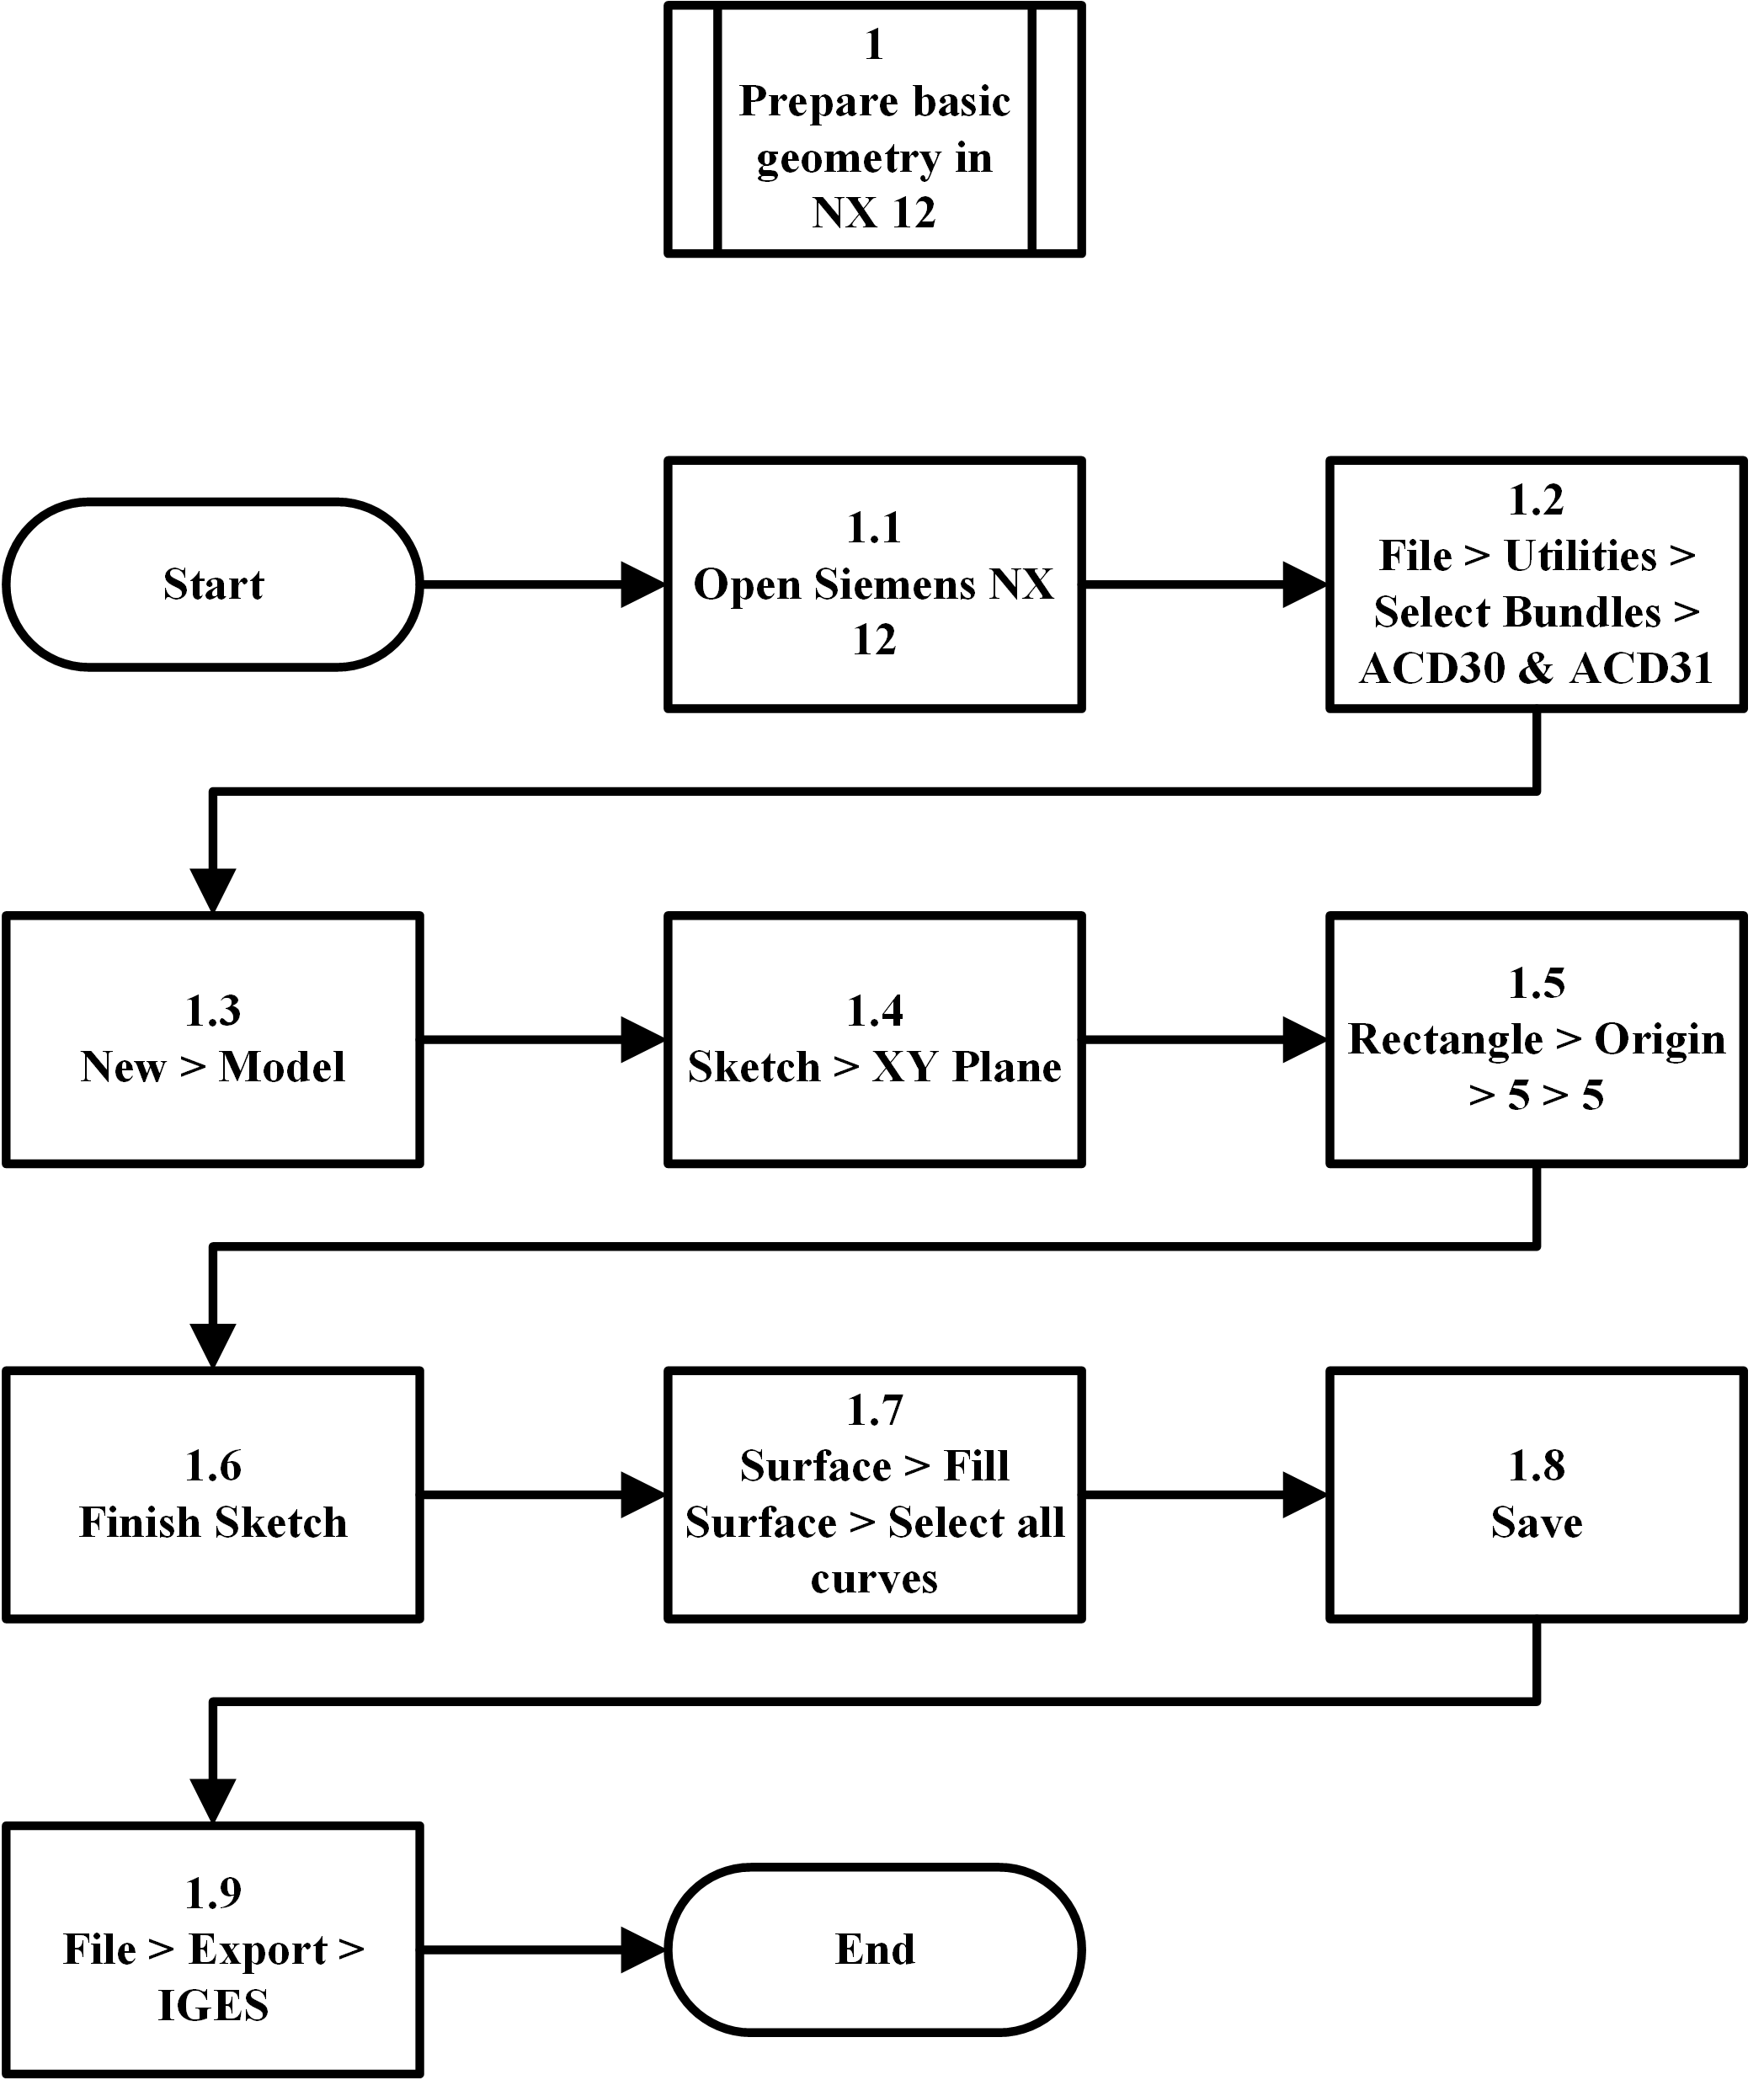
\includegraphics[width=1\textwidth]{Q1_1.png}
	\caption{Preparation of basic geometry in NX 12 flowchart}
	\label{fig:f1}
\end{figure}

\begin{figure}
	\includegraphics[width=1\textwidth]{Q1_3.png}
	\caption{Preparation of geometry in Marc Mentat flowchart}
	\label{fig:f3}
\end{figure}

\begin{table}
\centering
\caption{Pre-Automesh (3.6)}
\label{tab:f36}
\resizebox{\textwidth}{!}{%
\begin{tabular}{@{}llllcc@{}}
\toprule
\multicolumn{1}{c}{\textbf{Ribbon}} &
  \multicolumn{1}{c}{\textbf{Tab}} &
  \multicolumn{1}{c}{\textbf{Command}} &
  \multicolumn{1}{c}{\textbf{Input}} &
  \textbf{Target Length} &
  \textbf{\begin{tabular}[c]{@{}c@{}}Apply Curve\\ Divisions\end{tabular}} \\ \midrule
\begin{tabular}[c]{@{}l@{}}Geometry\\ \& Mesh\end{tabular} &
  Pre-Automesh &
  Curve Divisions &
  Target Length &
  1 &
  1 2 3 4 \\ \bottomrule
\end{tabular}%
}
\end{table}

\begin{table}
\centering
\caption{Automesh (3.7)}
\label{tab:f37}
\resizebox{\textwidth}{!}{%
\begin{tabular}{@{}llllc@{}}
\toprule
\multicolumn{1}{c}{\textbf{Ribbon}} &
  \multicolumn{1}{c}{\textbf{Tab}} &
  \multicolumn{1}{c}{\textbf{Command}} &
  \multicolumn{1}{c}{\textbf{Quadrilaterals (Adv Frnt)}} &
  \textbf{Enter curve list} \\ \midrule
Geometry \& Mesh &
  Automesh &
  Planar &
  Quad Mesh! &
  1 2 3 4 \\ \bottomrule
\end{tabular}%
}
\end{table}

\begin{table}
\centering
\caption{Tables (3.8)}
\label{tab:f38}
\resizebox{\textwidth}{!}{%
\begin{tabular}{@{}llllccc@{}}
\toprule
\multicolumn{1}{c}{\textbf{Ribbon}} &
  \multicolumn{1}{c}{\textbf{Tab}} &
  \multicolumn{1}{c}{\textbf{Command}} &
  \multicolumn{1}{c}{\textbf{Name}} &
  \multicolumn{2}{c}{\textbf{\begin{tabular}[c]{@{}c@{}}Independent\\ Variable V1\end{tabular}}} &
  \textbf{\begin{tabular}[c]{@{}c@{}}Function\\ Value F\end{tabular}} \\ \midrule
\multirow{2}{*}{\begin{tabular}[c]{@{}l@{}}Tables \&\\ Coord. Syst.\end{tabular}} &
  \multirow{2}{*}{Tables} &
  \multirow{2}{*}{\begin{tabular}[c]{@{}l@{}}New\\ \textgreater{}1 Independent Variable\end{tabular}} &
  \multirow{2}{*}{ramp} &
  \textbf{Type} &
  \textbf{Steps} &
  \textbf{Steps} \\ \cmidrule(l){5-7} 
 &
   &
   &
   &
  \multicolumn{1}{l}{time} &
  1 &
  1 \\ \bottomrule
\end{tabular}%
}
\end{table}

\begin{table}
\centering
\caption{Boundary Conditions - Displacement (3.9)}
\label{tab:f39}
\resizebox{\textwidth}{!}{%
\begin{tabular}{@{}llllccccccl@{}}
\toprule
\multicolumn{1}{c}{\textbf{Ribbon}} &
  \multicolumn{1}{c}{\textbf{Tab}} &
  \multicolumn{1}{c}{\textbf{Command}} &
  \multicolumn{1}{c}{\textbf{Name}} &
  \textbf{\begin{tabular}[c]{@{}c@{}}Displacement\\ X\end{tabular}} &
  \textbf{\begin{tabular}[c]{@{}c@{}}Displacement\\ Y\end{tabular}} &
  \textbf{\begin{tabular}[c]{@{}c@{}}Displacement\\ Z\end{tabular}} &
  \textbf{\begin{tabular}[c]{@{}c@{}}Rotation\\ X\end{tabular}} &
  \textbf{\begin{tabular}[c]{@{}c@{}}Rotation\\ Y\end{tabular}} &
  \textbf{\begin{tabular}[c]{@{}c@{}}Rotation\\ Z\end{tabular}} &
  \multicolumn{1}{c}{\textbf{Add Nodes}} \\ \midrule
\begin{tabular}[c]{@{}l@{}}Boundary\\ Conditions\end{tabular} &
  \begin{tabular}[c]{@{}l@{}}Boundary\\ Conditions\end{tabular} &
  \begin{tabular}[c]{@{}l@{}}New (Structural)\\ \textgreater Fixed Displacement\end{tabular} &
  fix &
  0 &
  0 &
  0 &
  0 &
  0 &
  0 &
  \begin{tabular}[c]{@{}l@{}}1 2 3 4 5 6\\ 16 17 18 19 20\end{tabular} \\ \bottomrule
\end{tabular}%
}
\end{table}

\begin{table}
\centering
\caption{Boundary Conditions - Load (3.10)}
\label{tab:f310}
\resizebox{\textwidth}{!}{%
\begin{tabular}{@{}llllclc@{}}
\toprule
\multicolumn{1}{c}{\textbf{Ribbon}} &
  \multicolumn{1}{c}{\textbf{Tab}} &
  \multicolumn{1}{c}{\textbf{Command}} &
  \multicolumn{1}{c}{\textbf{Name}} &
  \textbf{Pressure} &
  \multicolumn{1}{c}{\textbf{Table}} &
  \textbf{Add Curves} \\ \midrule
\begin{tabular}[c]{@{}l@{}}Boundary\\ Conditions\end{tabular} &
  \begin{tabular}[c]{@{}l@{}}Boundary\\ Conditions\end{tabular} &
  \begin{tabular}[c]{@{}l@{}}New (Structural) \\ \textgreater Edge Load\end{tabular} &
  load &
  -10 &
  ramp &
  2:0 3:0 \\ \bottomrule
\end{tabular}%
}
\end{table}

\begin{table}
\centering
\caption{Geometric Properties (3.11)}
\label{tab:f311}
\resizebox{\textwidth}{!}{%
\begin{tabular}{@{}lllll@{}}
\toprule
\multicolumn{1}{c}{\textbf{Ribbon}} &
  \multicolumn{1}{c}{\textbf{Tab}} &
  \multicolumn{1}{c}{\textbf{Command}} &
  \multicolumn{1}{c}{\textbf{Name}} &
  \multicolumn{1}{c}{\textbf{Add Elements}} \\ \midrule
Geometric Properties &
  Geometric Properties &
  \begin{tabular}[c]{@{}l@{}}New (Structural)\\ \textgreater Plane Strain\end{tabular} &
  straingeom &
  all \\ \bottomrule
\end{tabular}%
}
\end{table}

\begin{table}
\centering
\caption{Material Properties (3.12)}
\label{tab:f312}
\resizebox{\textwidth}{!}{%
\begin{tabular}{@{}lllllccl@{}}
\toprule
\multicolumn{1}{c}{\textbf{Ribbon}} &
  \multicolumn{1}{c}{\textbf{Tab}} &
  \multicolumn{1}{c}{\textbf{Command}} &
  \multicolumn{1}{c}{\textbf{Name}} &
  \multicolumn{1}{c}{\textbf{Type}} &
  \textbf{C10} &
  \textbf{C01} &
  \multicolumn{1}{c}{\textbf{Add Elements}} \\ \midrule
Material Properties &
  Material Properties &
  \begin{tabular}[c]{@{}l@{}}New\\ \textgreater Finite Stiffness Region\\ \textgreater Standard\end{tabular} &
  rubber &
  Mooney &
  20.3 &
  5.8 &
  all \\ \bottomrule
\end{tabular}%
}
\end{table}

\begin{table}
\centering
\caption{Loadcases (3.13)}
\label{tab:f313}
\begin{tabular}{@{}llllc@{}}
\toprule
\multicolumn{1}{c}{\textbf{Ribbon}} &
  \multicolumn{1}{c}{\textbf{Tab}} &
  \multicolumn{1}{c}{\textbf{Command}} &
  \multicolumn{1}{c}{\textbf{Name}} &
  \textbf{\# Steps} \\ \midrule
Loadcases &
  Loadcases &
  \begin{tabular}[c]{@{}l@{}}New\\ \textgreater Static\end{tabular} &
  pressureload &
  100 \\ \bottomrule
\end{tabular}
\end{table}

\begin{figure}
	\centering
	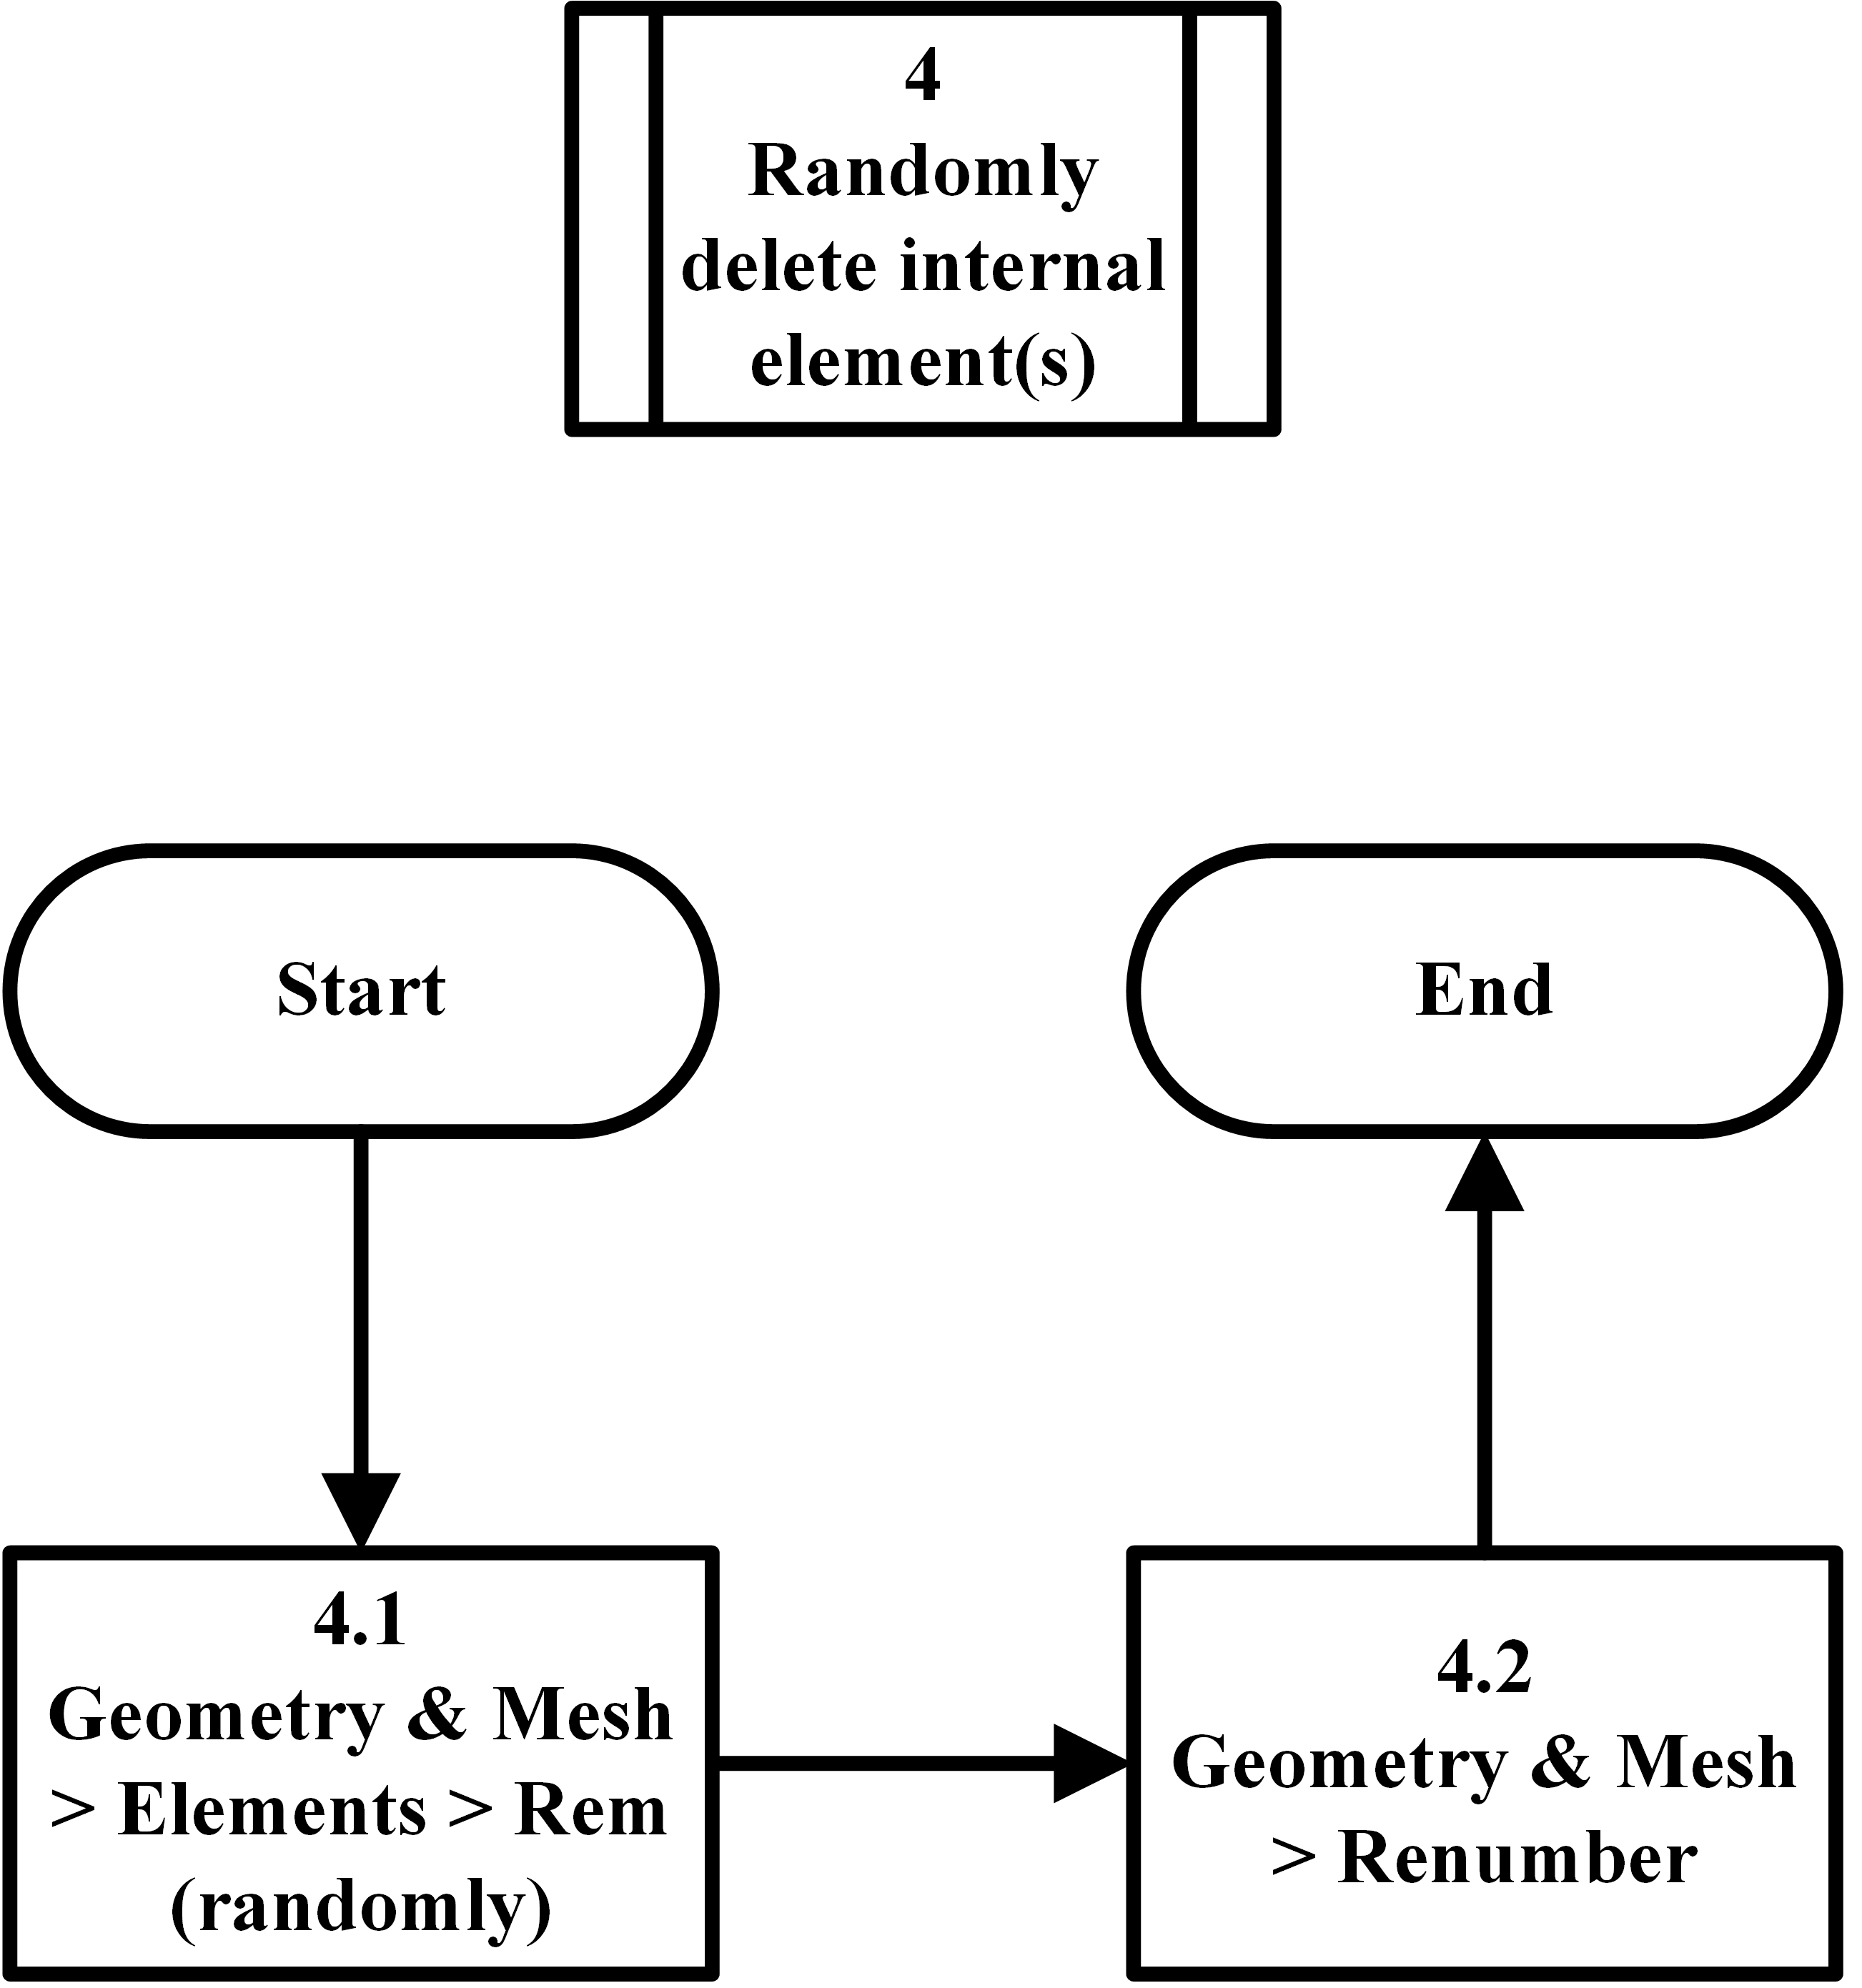
\includegraphics[width=0.66\textwidth]{Q1_4.png}
	\caption{Random deletion of internal element(s) flowchart}
	\label{fig:f4}
\end{figure}

\begin{table}
\centering
\caption{Element removal (4.1)}
\resizebox{\textwidth}{!}{%
\label{tab:f41}
\begin{tabular}{@{}lllc@{}}
\toprule
\multicolumn{1}{c}{\textbf{Ribbon}} & \multicolumn{1}{c}{\textbf{Tab}} & \multicolumn{1}{c}{\textbf{Command}} & \textbf{Rem Elements}   \\ \midrule
Geometry \& Mesh                    & Basic Manipulation               & Geometry \& Mesh                     & 7 8 9 12 13 14 17 18 19 \\ \bottomrule
\end{tabular}
}
\end{table}

\begin{table}
\centering
\caption{Renumber elements (4.2)}
\label{tab:f42}
\resizebox{\textwidth}{!}{%
\begin{tabular}{@{}llll@{}}
\toprule
\multicolumn{1}{c}{\textbf{Ribbon}} & \multicolumn{1}{c}{\textbf{Tab}} & \multicolumn{1}{c}{\textbf{Command}} & \multicolumn{1}{c}{\textbf{Command}} \\ \midrule
Geometry \& Mesh                    & Basic Manipulation               & Renumber                             & All Geometry \& Mesh                 \\ \bottomrule
\end{tabular}
}
\end{table}

\begin{figure}
	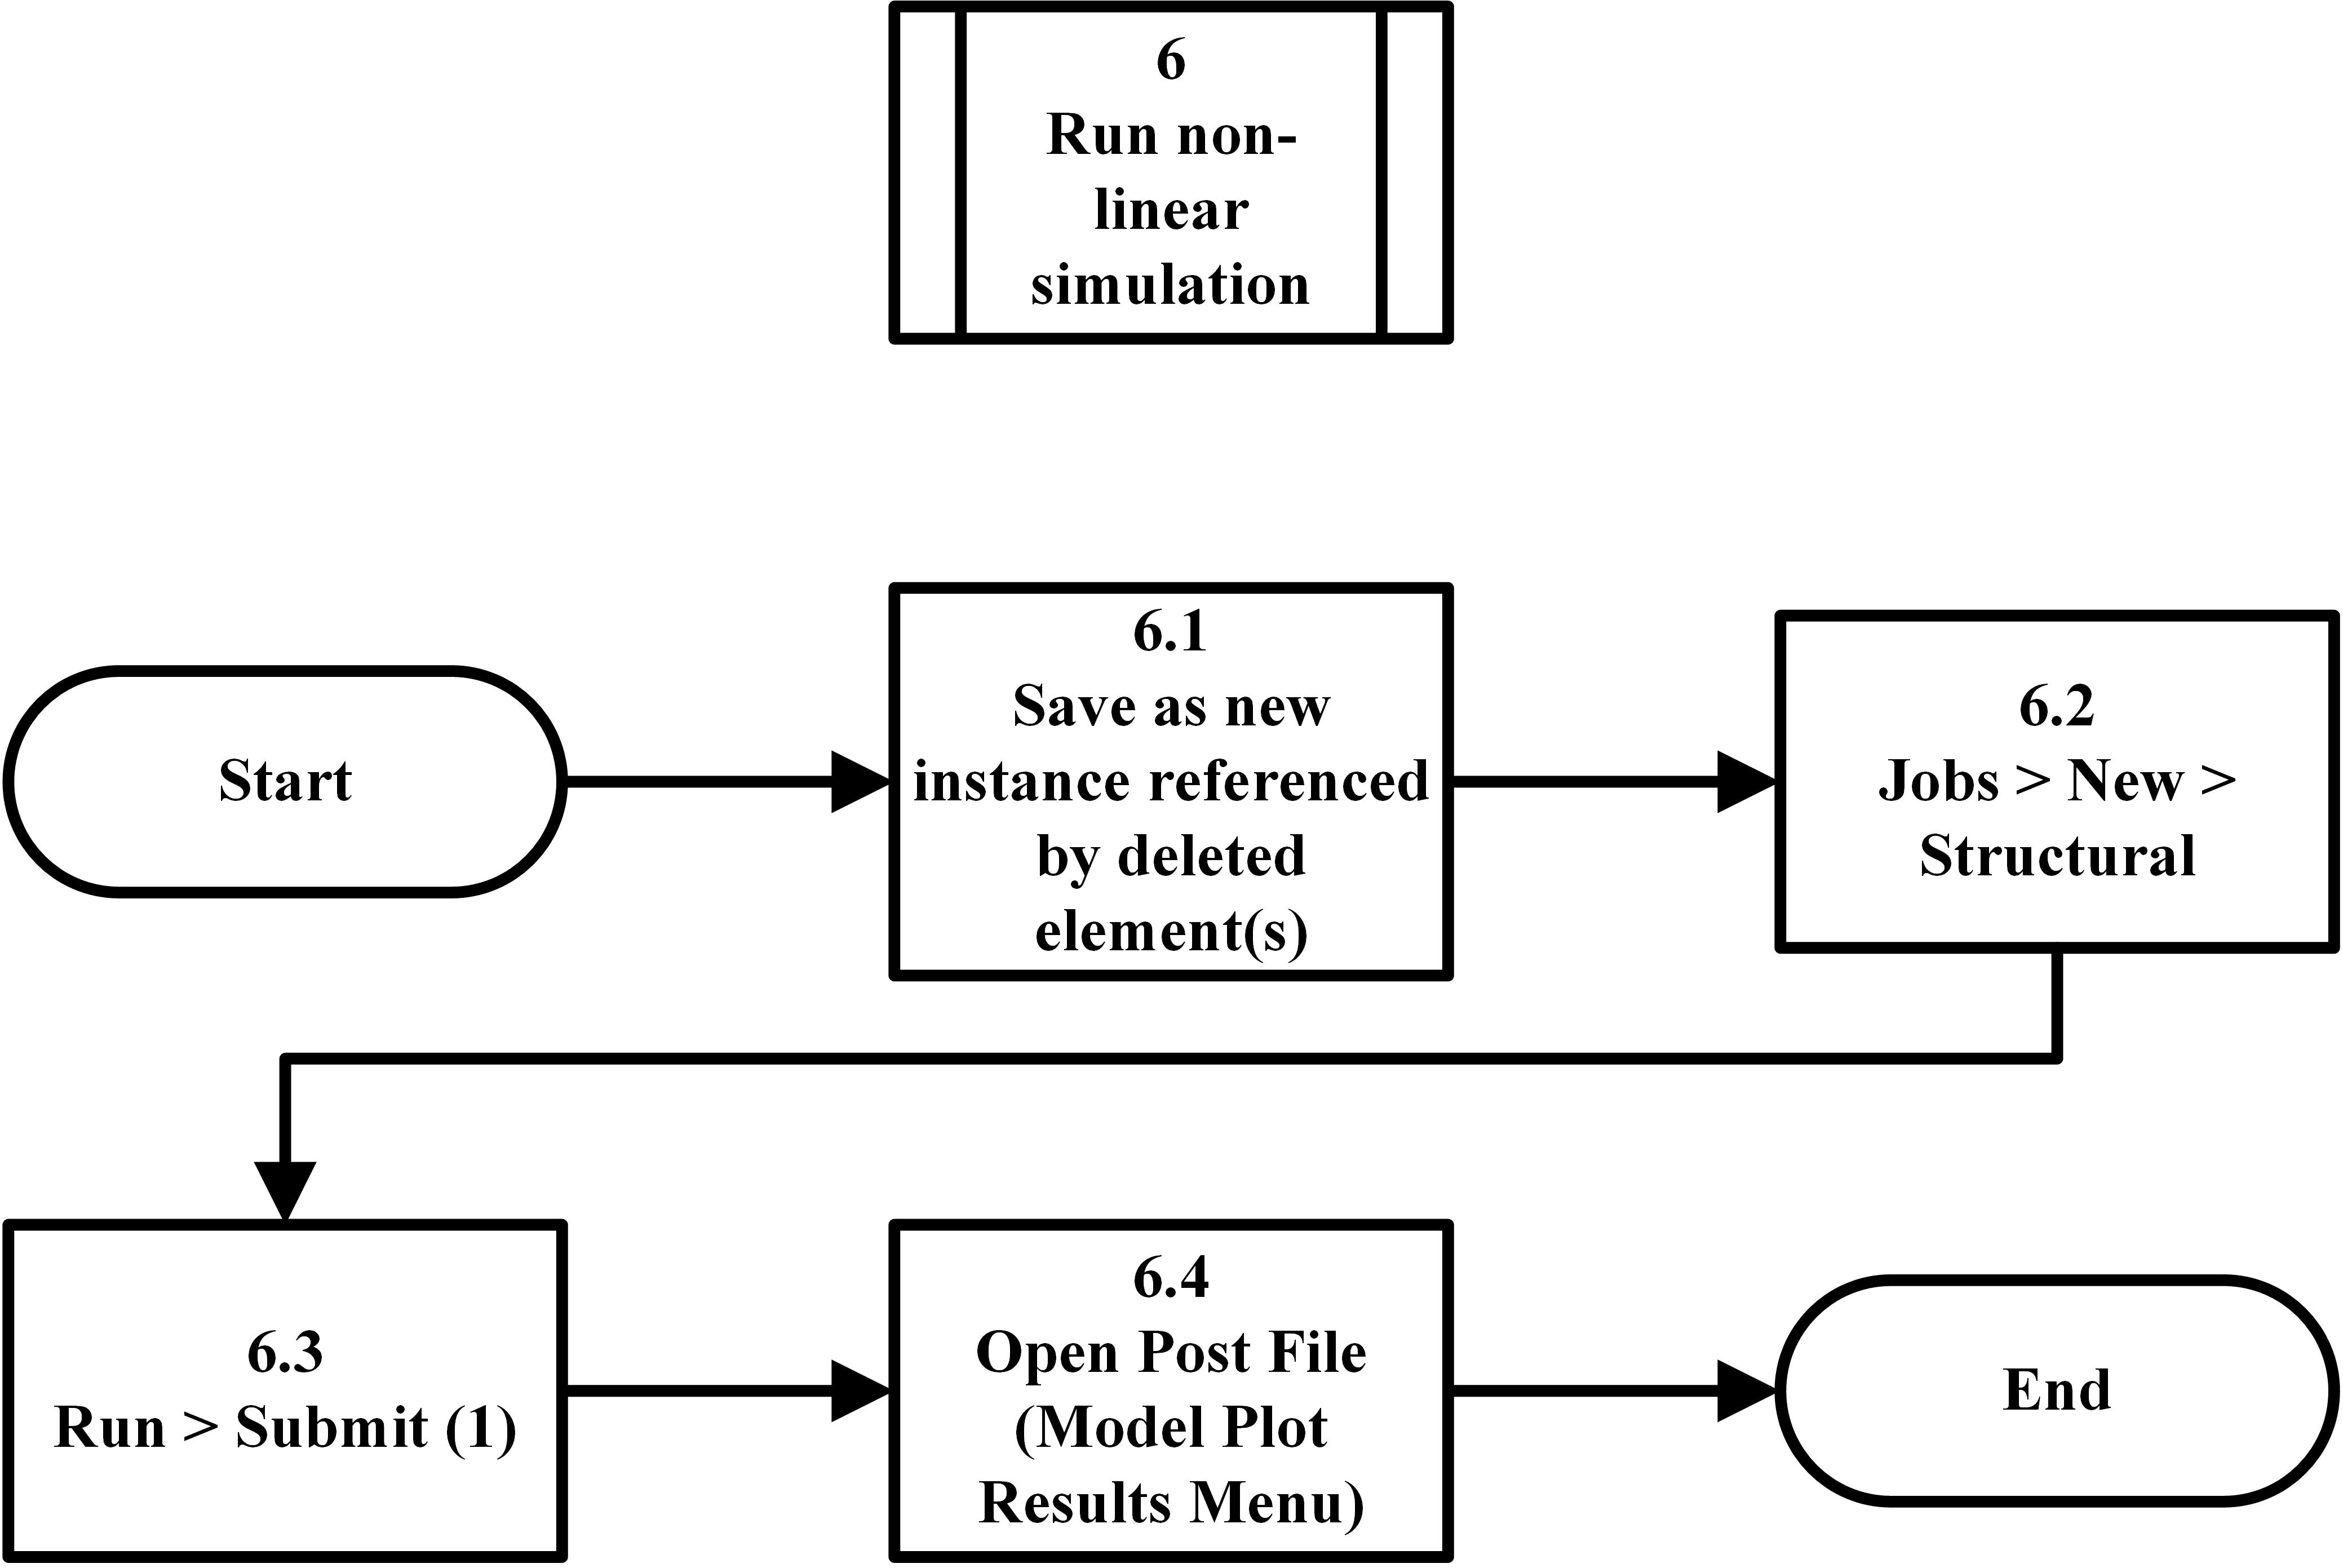
\includegraphics[width=1\textwidth]{Q1_6.png}
	\caption{Non-linear simulation flowchart}
	\label{fig:f6}
\end{figure}

\begin{table}
\centering
\caption{Jobs (6.2)}
\label{tab:f62}
\resizebox{\textwidth}{!}{%
\begin{tabular}{@{}lllllllcl@{}}
\toprule
\multicolumn{1}{c}{\textbf{Ribbon}} &
  \multicolumn{1}{c}{\textbf{Tab}} &
  \multicolumn{1}{c}{\textbf{Command}} &
  \multicolumn{1}{c}{\textbf{Name}} &
  \multicolumn{1}{c}{\textbf{Selected}} &
  \multicolumn{2}{c}{\textbf{\begin{tabular}[c]{@{}c@{}}Analysis\\ Options\end{tabular}}} &
  \multicolumn{2}{c}{\textbf{Job Results}} \\ \midrule
\multirow{2}{*}{Jobs} &
  \multirow{2}{*}{Jobs} &
  \multirow{2}{*}{\begin{tabular}[c]{@{}l@{}}New\\ \textgreater Structural\end{tabular}} &
  \multirow{2}{*}{job\_\textless{}deleted\_element(s)\textgreater{}} &
  \multirow{2}{*}{pressureload} &
  \multirow{2}{*}{\begin{tabular}[c]{@{}l@{}}Large\\ Strain\end{tabular}} &
  \multirow{2}{*}{\begin{tabular}[c]{@{}l@{}}Follower\\ Force\end{tabular}} &
  \multicolumn{2}{c}{\textbf{Available Element Scalars}} \\ \cmidrule(l){8-9} 
 &
   &
   &
   &
   &
   &
   &
  \multicolumn{1}{l}{\begin{tabular}[c]{@{}l@{}}Equivalent Von\\ Mises Stress\end{tabular}} &
  \begin{tabular}[c]{@{}l@{}}Total Strain \\ Energy\end{tabular} \\ \bottomrule
\end{tabular}%
}
\end{table}

\begin{figure}
	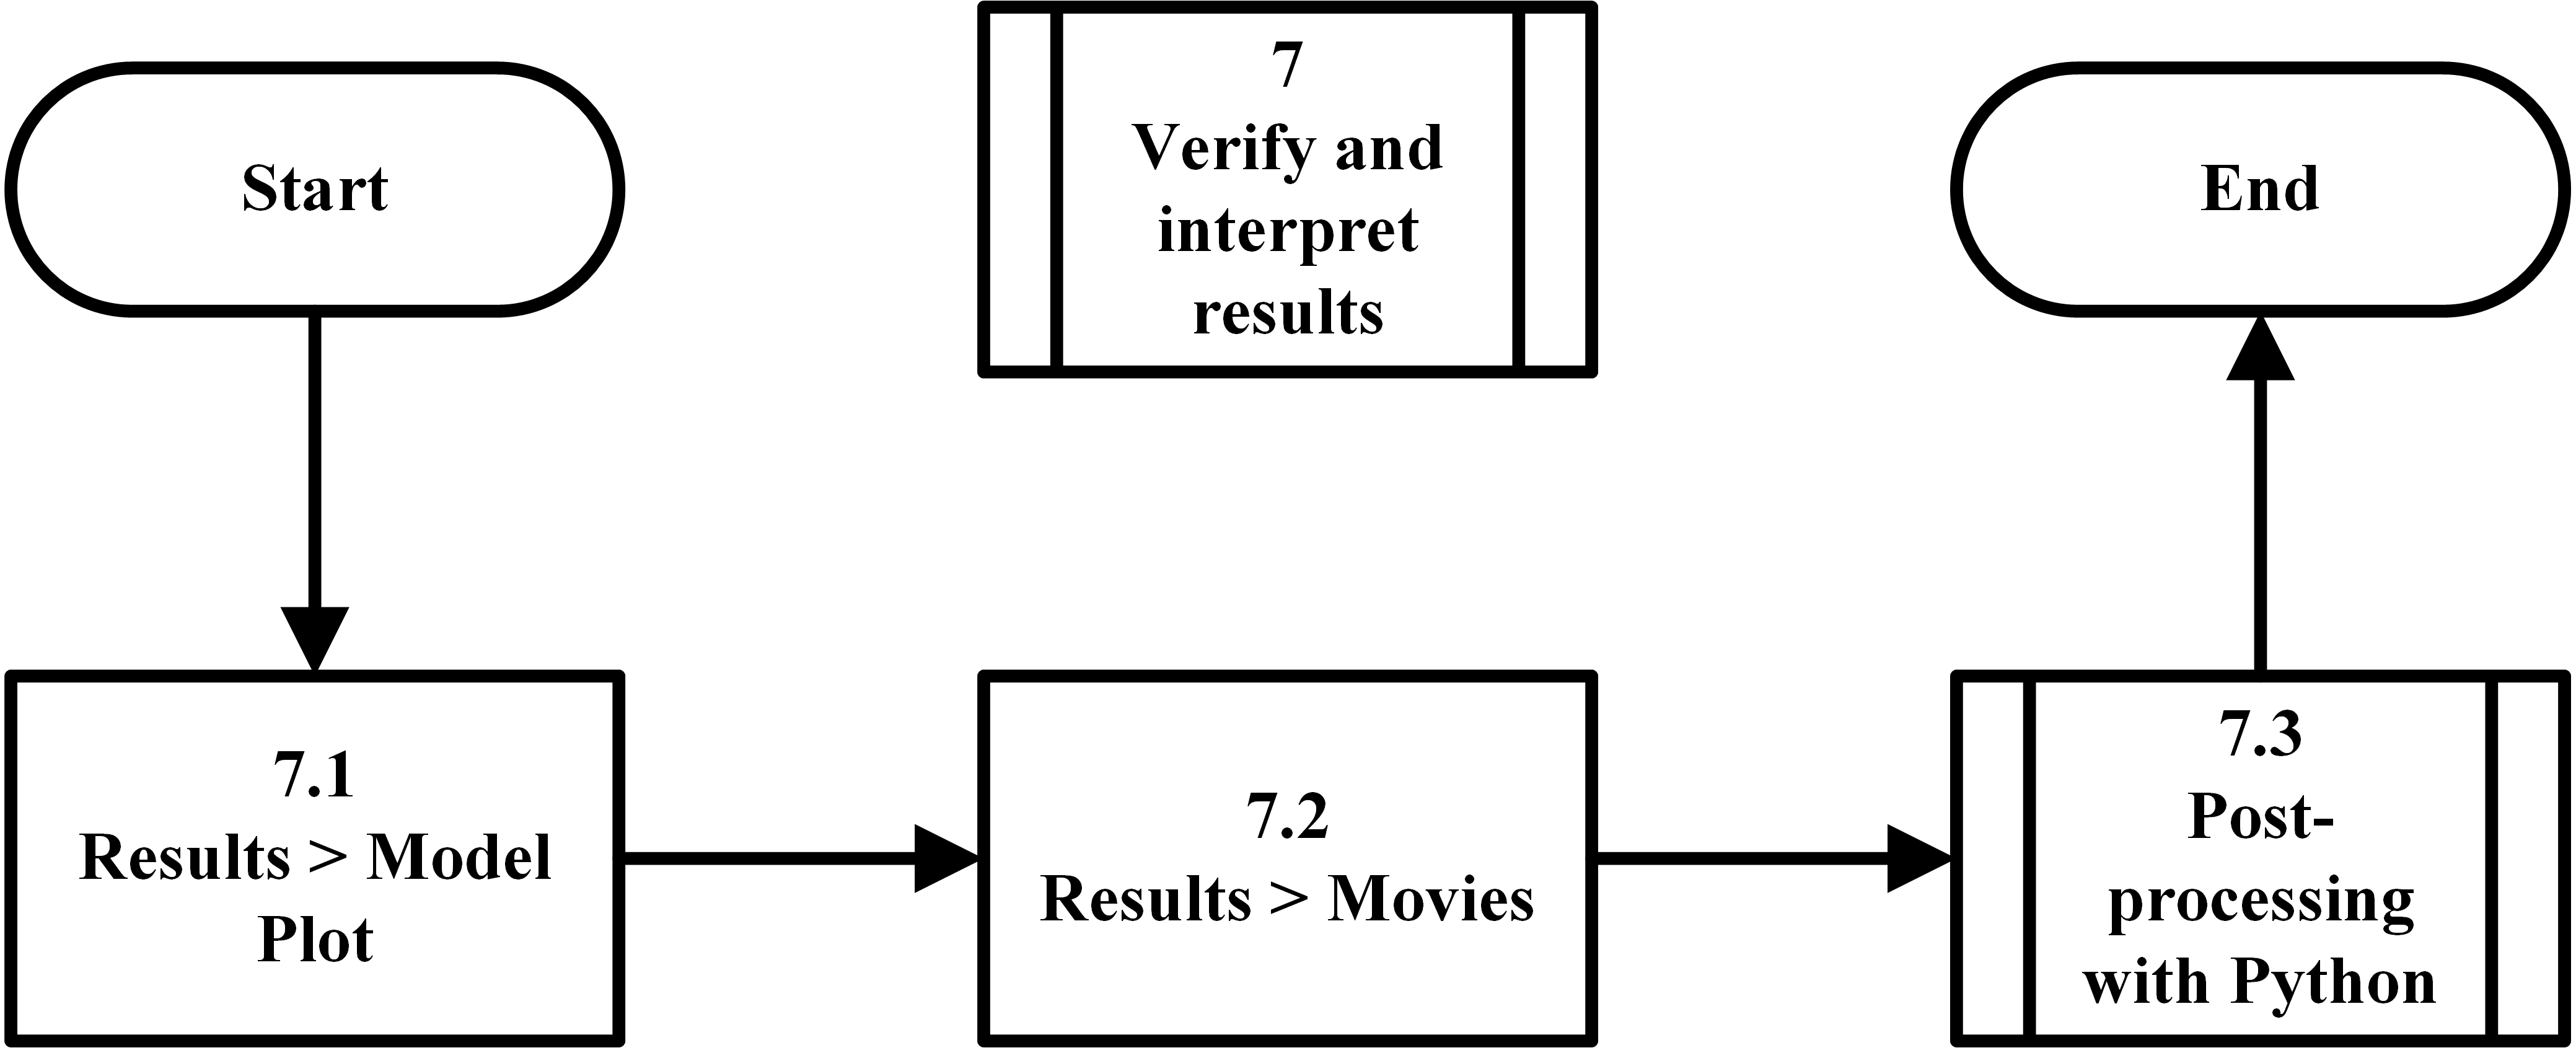
\includegraphics[width=1\textwidth]{Q1_7.png}
	\caption{Verification and interpretation of results flowchart}
	\label{fig:f7}
\end{figure}

\begin{table}
\centering
\caption{Model Plot (7.1)}
\label{tab:f71}
\resizebox{\textwidth}{!}{%
\begin{tabular}{@{}lllcl@{}}
\toprule
\multicolumn{1}{c}{\textbf{Ribbon}} &
  \multicolumn{1}{c}{\textbf{Command}} &
  \multicolumn{1}{c}{\textbf{Style}} &
  \multicolumn{2}{c}{\textbf{Scalar Plot}} \\ \midrule
\multirow{2}{*}{Results} &
  \multirow{2}{*}{Model Plot} &
  \multirow{2}{*}{Deformed \& Original} &
  \textbf{Style} &
  \multicolumn{1}{c}{\textbf{Scalar}} \\ \cmidrule(l){4-5} 
 &
   &
   &
  \multicolumn{1}{l}{Contour Bands} &
  Total Strain Energy \\ \bottomrule
\end{tabular}
}
\end{table}

\begin{table}
\centering
\caption{Movies (7.2)}
\label{tab:f72}
\resizebox{\textwidth}{!}{%
\begin{tabular}{@{}llll@{}}
\toprule
\multicolumn{1}{c}{\textbf{Ribbon}} &
  \multicolumn{1}{c}{\textbf{Command}} &
  \multicolumn{1}{c}{\textbf{Base File Name}} &
  \multicolumn{1}{c}{\textbf{Command}} \\ \midrule
Results &
  Movies &
  baseelement\_\textless{}deleted\_element(s)\textgreater{} &
  Make GIF Movie \\ \bottomrule
\end{tabular}
}
\end{table}